\documentclass[a4paper,11pt]{article}

%-------------------------------------------------------------------------------
%--- (a) Required Packages
%-------------------------------------------------------------------------------
\usepackage{amsmath,amsfonts,amssymb,amsthm}
\usepackage{adjustbox}
\usepackage{subcaption}
\usepackage{subfloat}
\usepackage{mwe}
\usepackage{authblk}
\usepackage[english]{babel}
\usepackage{lscape}
\usepackage{tabu}
\usepackage{bm}
\usepackage{booktabs}
\usepackage{caption}
\usepackage[usenames, dvipsnames]{color}
\usepackage{epstopdf}
%\usepackage[capposition=top]{floatrow}
\usepackage{framed}
%\usepackage[T1]{fontenc}
\usepackage{lmodern}
\usepackage{graphicx}
\usepackage{hyperref}
\usepackage[utf8]{inputenc}
\usepackage{natbib}
\usepackage{setspace}
\usepackage{rotating}
\usepackage{url}
\usepackage{multicol}
\usepackage[toc,page]{appendix}
\usepackage{float}
\interfootnotelinepenalty=10000
\usepackage[margin=1in,footskip=0.25in]{geometry}
\usepackage{longtable}
\usepackage{babel,blindtext}

%-------------------------------------------------------------------------------
%--- (b) Specific margins
%-------------------------------------------------------------------------------
%\setlength  \textwidth{\paperwidth}
%\setlength  \textheight{\paperheight}
%\setlength  \oddsidemargin{3cm}
%\setlength  \topmargin{-1.2cm}
%\setlength  \footnotesep{2ex}
%\addtolength\textheight{-6cm}
%\addtolength\textwidth{-6cm}
%\addtolength\oddsidemargin{-1in}
\setlength\parskip{0.25in} 
 
%%ADDED SPACE BETWEEN PARAGRAPHS 
%-------------------------------------------------------------------------------
%--- (c) Internal Ref stype
%-------------------------------------------------------------------------------
\hypersetup{            
    colorlinks=true,   
    linkcolor=Black,
    citecolor=BlueViolet,
    filecolor=BlueViolet,
    urlcolor=Black
}


 
%-------------------------------------------------------------------------------
%--- (1) Title
%-------------------------------------------------------------------------------
\title{\textsc{the impact of abortion legalization on fertility and female empowerment: new evidence from mexico}\thanks{We are grateful to Andreea Mitrut, Randi Hjalmarsson, Elin Larsson, Blair G. Darney, Hans Gr\"onqvist and seminar audiences at the Department of Economics at University of Gothenburg,  SOFI Stockholm University, Karolinska Institute and the CSAE conference for their very useful comments and discussions.  We thank Alejandro del Valle for sharing data, and Susanna Lindahl for excellent research assistance.}}
\author{Damian Clarke\thanks{Department of Economics, Universidad de Santiago de Chile.  Contact: damian.clarke@usach.cl} \hspace{1cm} Hanna Mühlrad\thanks{Department of Economics, University of Gothenburg. Contact: hanna.muhlrad@gu.se}}


%-------------------------------------------------------------------------------
%---  ABSTACT
%-------------------------------------------------------------------------------
\begin{document}
\pagenumbering{gobble}
\maketitle
%\newpage
\pagenumbering{arabic}

\begin{spacing}{1.5}
%\begin{center}
%  {\Large The Impact of Abortion Legalization on Fertility and Maternal Mortality: New Evidence from Mexico}
%  \\
%\vspace{5mm}
%  \textbf{Running Title}: Abortion Legalization, Fertility and Maternal Death \\
%\textbf{Keywords:} Fertility, Maternal Mortality, Abortion legalization, Mexico

%\end{center}

%\newpage

\begin{abstract}
\noindent We examine the effect of a large-scale, free, elective abortion program implemented in Mexico City in 2007. Prior to this program, all states and districts in Mexico had very limited, or no, access to elective abortion. A localized reform in Mexico City resulted in a sharp increase in the request and use of early term elective abortions: approximately 90,000 abortions were administered by public health providers in the four years following the reform, versus only 62 in the five years preceding the reform. 
\end{abstract}
\textbf{Keywords:} Fertility, Female Empowerment, Abortion legalization, Mexico \\
\noindent \hspace{7mm} \textbf{JEL Codes:} J13, I15, I18, O15. 
\end{spacing}

%-------------------------------------------------------------------------------
%---  INTRODUCTION
%-------------------------------------------------------------------------------
\newpage 
\begin{spacing}{1.5}

\section{Introduction}
The issue of abortion legalization continues to be a highly controversial social topic.  This is especially true in Latin America, which has some of the world's most rigid abortion laws \citep{UN2014} as well as the highest estimated rates of unsafe abortions in the world, with 31 abortions per 1,000 fertile-aged women compared to the worldwide rate of 14 per 1,000 women. The high number of unsafe abortions in the Latin American and Caribbean (LAC) region corresponds to an estimated 4.2 million unsafe induced abortions each year, and 12\% of all maternal deaths in the region \citep{WHO2011}.

The ongoing public debate on abortion legalization continues to flare, not least in connection with the recent outbreak in Brazil of the ``\textit{Zika virus}'', which is thought to lead to microcephaly among infants \citep{heymann2016zika}. Some groups of lawyers, doctors, activists and UN spokesperson Cecile Pouilly have called on the Supreme Court of Brazil to allow for induced abortions \citep{guardianFeb}. When looking at the LAC region, there has been a development towards a more liberal abortion legislation in several South American countries, while opposite trends have followed in Central America (see \cite{Fraser2015} for an extended discussion). Similarly, differences in abortion laws can also be found on a sub-national level, which is the case for Mexico City where elective abortion during the first trimester was legalized in 2007.


In this study, we examine the effect of a sharply defined local abortion reform in Mexico City and document the effect of free access to legal and safe abortion services on fertility, sexual behaviour and female empowerment. We combine the state-level variation over time resulting from this natural experiment with high quality vital statistics data on 23 millions of births.  This reform---the so called legal interruption of pregnancy (or ILE for its name in Spanish)---was of considerable importance.  During the pre-reform period of 2001-2007 a total of 62 legal abortions (available in restrictive conditions) were performed in Mexico City.  Following the 2007 reform, more than 90,000 women accessed safe legal abortion between 2008 and 2012.

Abortion laws are determined at the state level in Mexico, where Mexico City (also known as the federal district of Mexico) has its own legislative assembly.  The ILE reform provided all women who reside in Mexico City with access to legal and safe abortion procedures, free of charge and for any reason, during the first trimester of pregnancy. The law was a radical change from previous legislation in Mexico City, and also compared to the rest of the states of Mexico, where abortion is still banned in all but the extreme circumstances of rape, to save the mother's life, or in cases of severe fetal malformation.\footnote{Depending on the state, these circumstances include none, some, or all of rape, fetal inviability or grave danger to the health of the mother. One exception is the state of Yucatan, which, since 1931, has permitted legally induced abortions for socio-economic reasons for women with at least three children \citep{GIRE2009}.} Moreover, by legalizing abortion, Mexico City distinguishes itself from nearly all other countries in Latin America and the Caribbean which remain highly restrictive in their policies related to elective abortion \citep{Fraser2015}.\footnote{According to the most recent United Nations figures \citep{UN2014}, Mexico is one of only three countries in the LAC region (along with Uruguay and Guyana) to be classified as the ``Least restrictive'' in abortion policy, implying that abortions are permitted for economic or social reasons upon request.}


 [Contribution here]

  Moreover, this is the first study to evaluate the overall effect on both fertility and maternal mortality from the 2007 abortion reform in Mexico City using the full set of available vital statistics for the period 2002-2011. This is, however, not the first study of the effect of Mexico's 2007 abortion reform.  A considerable academic literature exists across the fields of law \citep{Johnson2013}, public health \citep{Contreras2011,Schiavonetal2010,Becker2013,Kalb} and medicine \citep{Madrazo2009}.  It is, however, the first comprehensive analysis of the reform's effect using the full power of the vital statistics data.  Other existing studies either use infrequent registers and focus only on fertility \citep{Gutierrez2015}...  Many previous studies examine the effect of abortion legalization that took place in conjunction with other major laws and reforms. In contrast to those studies, contraception has been legal and freely provided by the government since 1974 in Mexico.

%All told, the results from this study suggest that the April 2007 abortion reform in Mexico City is associated with an important reduction in fertility and maternal mortality. These results are highly relevant when considering the achievement of international development goals, including the Sustainable Development Goals (SDGs), which require a two thirds reduction in maternal deaths world-wide by the year 2030.


%%%COPIED FROM LITERATURE BELOW
%%There is a growing body of literature regarding reproductive health policies within economics. Abortion policy is a topic that has gained ground during recent decades, providing evidence of both short and long term consequences from abortion legalization and decriminalization. Within economics, there are a few proposed theoretical frameworks analyzing abortion policies and multiple empirical studies usually based on quasi-experimental methods.\footnote{From a theoretical point of view, suggested by \cite{levine2004abortion} and \cite{ananat_abortion_2009}, fertility decisions can be viewed as sequential choices of first becoming pregnant and then whether or not to give birth. Access to legal and safe abortion procedures decreases the “cost” of interrupting a pregnancy. This can imply two different effects on fertility decisions. First, better access to abortion reduces the probability of birth ex post becoming pregnant. Second, improved access to abortion can alter ex ante behavior and thus positively affect the number of pregnancies since opting out from pregnancy is less costly. However, due to lack of data on abortions prior to legalization of abortion, most studies analyze the effect on overall fertility while fewer study behavioral responses. In another theoretical paper by \cite{akerlof1996analysis}, the implication of legalizing abortion (and contraception)  is examined. They argue that abortion legalization causes more out-of wedlock births due to less shot-gun marriages. \cite{chiappori2008birth} provide a theoretical model and show, in contrast to \cite{akerlof1996analysis}, that access to birth control methods (including abortion) increases women's welfare and ``power''.} There are several studies with empirical evidence showing that abortion legalization has a negative effect on birth rates. One of the most studied abortion policies, is the US Supreme Court decision in the 1970s (Roe \emph{v.}\ Wade) legalizing elective abortion in all states.\footnote{See for instance \cite{ananat_abortion_2009}, \cite{AngristEvans}, \cite{DonohueLevitt2001}, \cite{CharlesStephens2002}} As a result of legalizing elective abortion, fertility decreased by 5\% with a particularly strong effect on teenage fertility, which declined by 12\% (see \cite{levine2004} for review). 

%%Similarly, a negative impact on fertility has also been found in former Soviet countries in Eastern Europe \citep{levine2004abortion}. Among these studies are \cite{Pop-Eleches}, who studied the 1966 Romanian ban on abortion during the rule of the communist dictator Ceausescu. The results show a radical increase in the total fertility rate (from 1.9 in 1966 to 3.7 children the year after). In contrast to the evidence from the US reform, women most inclined to access abortions before the ban were women with high socio-economic status. Analogous to previous findings, a large decrease in fertility by 8\% was found in Nepal when legalizing abortion \citep{Valente2010}.\footnote{In addition to short run effects, several papers examine the long run effect of abortion policies. From the US abortion policy, improved health and labor market outcomes have been found for the second generation. For instance, studies show improved outcomes in terms of lower child morbidity and mortality \citep{Gruberetal}, sharp decline in criminality \citep{DonohueLevitt2001}, more schooling and less welfare recipients \citep{ananat_abortion_2009} and reduced risk of substance abuse amongst adults \citep{CharlesStephens2002}. Similar results are found in Romania for the second generation. When controlling for various background covariates, infant mortality as well as later in life outcomes are worse for children born after the ban compared to those born prior \citep{Pop-Eleches} and \citep{Mitrut2011}.}



%There are a number of studies which analyze the impact of the abortion legalization in Mexico using national vital statistics; . Regarding the abortion reform and fertility outcomes, \cite{Gutierrez2015} use national vital statistics to examine the effect on fertility across ages. Due to the use of a limited amount of data and limitations inherent in the empirical design one cannot assign a causal interpretation to the results with confidence.\footnote{Only a limited amount of data is used comparing outcomes between three different years (1990, 2000 and 2010). Particularly, their ``double-difference'' coefficient is a simple comparison between 1990-2000 and 2000-2010, which is not a consistent way of using a difference in difference method (see for instance \cite{wooldridge2010econometric}), especially because the treatment group in not correctly specified when using the entire period 2000-2010 as the post treatment period while the reform took place in 2007} On the topic of the relationship between abortion legislation and maternal mortality in Mexico for the time period 2002-2011, \cite{Koch01022015} use national vital statistics and compare maternal mortality across states with ``less or more permissive'' abortion laws. However, the definition regarding ``less or more permissive'' abortion laws, used in  \cite{Koch01022015} leads to a misleading conclusion regarding the causal link between abortion legalization and maternal mortality.\footnote{Firstly, the treatment and control groups are incorrectly specified since the definition of abortion laws being “less or more permissive” are considered arbitrarily chosen (since abortion is only accessible in Mexico City and highly restricted elsewhere \citep{Kulczycki2011}). Secondly, \cite{Koch01022015} fail to account for lagged reporting of births by INEGI, resulting in more than 3 million incorrectly included births that took place before 2002. Thirdly, there is lacking information on the specification which has been used in this study. It does however appear that the treatment area is simply compared to the control area without using any methods that would provide results with a causal interpretation.} 


\section{Mexican Context and the ILE Reform}
\label{reform}
Fertility and abortion in the Mexican context. Unintended pregnancies lead to a worldwide number of approximately 46 million induced abortions each year \citep{van2005world}. Induced abortion is a procedure or medical treatment for terminating pregnancy. While induced abortion under safe settings is considered one of the safest medical procedures in modern medicine, unsafe abortion is associated with substantially increased risks of severe morbidity and mortality.\footnote{Induced abortions in a safe setting are carried out by professional health care providers in safe environment and in line with evidence based medicine. The procedure generally depends on gestational length of pregnancy. A safe induced abortion usually entails either a surgical operation or medical procedure. During a surgical operation, the products of conception are removed from the womb. The medical procedure is a non-invasive procedure that causes contractions of the womb, terminating the pregnancy. Medical abortion procedures are safer and more cost-efficient compared to other methods for first trimester abortions. It is common that the patient self-administers the medical abortion at home \citep{kulier2007medical}. Induced abortion under safe conditions exhibits a mortality rate below 1 per 100,000 procedures \citep{grimes2005risks}. } Unsafe abortion accounts for approximately 50\% of all induced abortions \citep{van2005world} and is defined by the WHO as ``a procedure for terminating a pregnancy performed by persons lacking the necessary skills or in an environment not in conformity with minimal medical standards, or both'' \citep{ganatra2014concept}. Breathtaking figures suggest that world-wide, unsafe abortions may result in as many as 8 maternal deaths per hour \citep{TheLancet2009}.  By the best available estimates, 13\% of all maternal deaths are due to complications surrounding clandestine and unsafe abortion, with these numbers being much higher in certain regions and groups \citep{WHO2011}.

The highest estimated rate of unsafe abortion occurs in the Latin America and Caribbean (LAC) region. Each year, an estimated 4.2 million unsafe induced abortions are carried out accounting for 12\% of all maternal deaths in the region \citep{WHO2011}. This region also exhibits some of the world’s most conservative laws on abortion \citep{UN2014}. Coherently with most countries in this region, Mexico has, until the legalization of abortion in Mexico City in 2007, had very strict legal restriction on access to abortion. Mexico consists of 32 federal entities, 31 of which are federal states plus the federal district of Mexico (also known as Mexico D.F.\ or Mexico City).  In addition to the national constitution, each of the 32 federal entities has its own state or local constitution, defined by its own legislative power. Abortion laws in all of Mexico are determined at the state level \citep{Becker2013}. Mexico City contains approximately 8\% of the entire population (8.9 million of Mexico's 119.5 million inhabitants according to 2015 estimates) and, since 2007, is the only state that allows for elective abortion during the first trimester.

Between the years 1975 and 2015, the fertility rate in Mexico declined rapidly from roughly 6 children per woman to approximately 2.2 children per woman. This major shift in fertility can be partially attributed to changes in access to modern contraceptive methods in the country \citep{GIRE2009}.  In 1975, the Mexican government passed the General Population Law, which obliged the government to supply family planning services and provide contraceptives via the public health care sector free of charge. In 1995, family planning services were decentralized to state level, where different states fund family planning to various degrees, possibly making family planning services differently available across states \citep{GIRE2009}.  Although 67\% of all women of childbearing age in Mexico report using modern contraceptive methods (and 5\% use traditional and less efficient methods)\footnote{Modern contraceptives are condoms, oral or/injectable/implants of hormones preventing ovulation, IUD, sterilization and emergency contraception. Traditional or less efficient methods are calendar method or rhythm method, coitus interrupts, herbs or teas. For a detailed account of modern and traditional methods, see for instance WHO: \url{http://www.who.int/mediacentre/factsheets/fs351/en/}}, it is estimated that more than half of all pregnancies are unintended. Estimates suggest that up to 54\% of these unintended pregnancies are terminated \citep{GIRE2009}. As a result, 54\% of these unintended pregnancies are terminated (Juarez et al., 2013).

Legal Restrictions. Prior to the reform in Mexico City, abortion laws were rather uniform across the 32 federal entities of Mexico. Induced abortion continues to be considered a criminal offense with the risk of up to 30 years imprisonment in many states \citep{GIRE2009}, and legal abortion was only permitted in the limited cases of rape, threat to the life of the mother, or severe malformation of the fetus.  In practice, even in these limited cases, legal abortion has been described by human rights organizations as extremely difficult to access due to rigid legal barriers \citep{GIRE2009}. In the densely populated Mexico City, only 62 abortions were legally performed during 2001-2007 \citep{Becker2013}.

Legal restrictions do not prevent induced abortions. The estimated rate of induced abortion in 2006 was 33 abortions per 1,000 women of fertile age \citep{ juarez2008estimates}, which is considered high internationally \citep{Becker2013}. As a substitute to legal options, abortions were performed in clandestine and often unsafe settings. In 2006 alone, medical records from public hospitals show that an estimated 150,000 women in Mexico were treated for abortion-related complications \citep{ juarez2008estimates}. Due to the illegal status of induced abortions, data on abortions is limited. The most common method of induced abortion is believed to be the abortifacient drug called Misoprostol account for approximately 30\% of all procedures\citep{GIRE2009}, which despite the of strict legal restrictions in Mexico, has been available in pharmacies in Mexico since 1985 \citep{lara2011often}. \footnote{Misoprostol (sometimes referred to as Cytotec, Arthrotec, Oxaprost, Cyprostol, Mibetec, Prostokos or Misotrol) is one of the recommended substance for induced abortion by the WHO \citep{lara2011often}. Misoprostol is a prostaglandin with the original purpose of curing gastric ulcers. It is also utilized for OB/GYN reasons such as induced abortion, post abortion procedures and induced labor for delivery\citep{kulier2007medical}.} Despite the fact Misoprostol and other abortifacients formally require a doctor's prescription in Mexico, studies show that abortifacients are frequently vended over the counter without prescription \citep{lara2011often}.  However, full and comprehensive instructions on dosage and usage of Misoprostol is generally not available at pharmacies \citep{lara2011often}. While Misoprostol is an efficient and well recognized method for induced abortion, the lack of knowledge about optimal use is assumed to result in complications for over 30\% of all cases \citep{GIRE2009}. The remaining two thirds of all induced abortions are believed not to include Misoprostol where 23\% are provided by doctors, 7\% by midwifes and nursed, 11\% by pharmacy workers and 14\% by traditional health providers. It is very difficult to estimate the cost and quality of different kinds of illegal abortion services, however, self-induced abortions without Misoprostol are considered the most unsafe procedures, which is thought to account for 16\% of all induced abortions.\footnote{See \cite{grimes2005risks} for detailed information on self-induced abortion procedures.} Unsafe abortions are more prevalent among poor women \citep{GIRE2009}, where the safety of the procedure usually depends on cost of the abortion service.  For instance, a safe illegal surgical abortion provided by a doctor at a private clinic in Mexico is estimated to cost between 404–660 US dollars. This can be compared to the monthly minimum wage of 132 US dollars \citep{GIRE2009}. Hence, it’s especially difficult for poor women to access safe induced abortion services making them extra exposed to severe complications and mortality \citep{GIRE2009}.

Due to the high number of unsafe abortions as well as a growing movement for women's reproductive health rights and a coalition of pro-choice NGO’s, the legislative assembly of the Federal District of Mexico City voted to legalize elective abortion (termed legal interruption of pregnancy, or ILE for its name in Spanish) on April 24, 2007, reforming Articles 145-148 of the penal code of Mexico City, and Article 14 of the Health Code.  These reforms were signed into law the following day, and published in the official Gazette of the Federal District on April 26, 2007 \citep{Gacetta2007}.  A broader discussion of the reform's social and legal setting is provided in \citet{Kulczycki2011, Madrazo2009}, \citep{blanco2011implementation} and \citet{Johnson2013}.  This immediately permitted women above the age of 18 to request legal interruption of pregnancy at up to 12 weeks of gestation without restriction.  Access for minors requires parental or guardian consent. Under this law, induced abortion where made legal in both public and private health care sector.

Implementation. Immediate implementation were made possible by collaboration between the Ministry of Health of Mexico City, members of the health department and international NGO’s , which had been thoroughly designed a program for public provision of abortion services called the ``the ILE program’’ and its implementation even before the law was passed \citep{singh2012making}.  NGO’s such as the International Pregnancy Advisory Services (IPAS) played a key role in implementing the ILE program in the public sector, providing both medical training to health care professionals as well as working with attitudes toward abortion \citep{blanco2011implementation}. As such, abortion services were made available via the public health care hospitals immediately after the law was passed in April 2007, although with lower capacity and efficiency compared to today. Abortion services were also quickly available in the private health care sector \citep{blanco2011implementation}.  Additionally, under this law sexual education in schools was improved, and post-abortion contraceptives were made freely available directly from the health clinics which provided abortions \citep{Contreras2011}. Records from public hospitals show that the demand for post-abortion contraceptives is high (approximately 82\% of all women accept contraceptives) and that prevalence of repeated abortion procedures are low \citep{Becker2013}.

On August 29 in 2008 the decision to pass the ILE law was ratified by the Supreme Court of Mexico. The abortion reform in Mexico City is distinguishable as a major social and political reform and makes Mexico City, together with Cuba and Uruguay, the most liberal jurisdiction in terms of abortion legislation in the entire Latin American and Caribbean region \citep{Fraser2015}.

Under the ILE program, women above age 18 with residency if Mexico City is offered abortion services free of charge at a selected number of public health clinics operated via the Ministry of Health in Mexico City (MOH-DF)\footnote{The public health care sector in Mexico is divided at both federal and state level, where the Ministry of Health (MOH) in Mexico City provides abortion procedures at a selected number of MOH-DF hospitals. Other MOH facilities (federally or state funded) are not legally required to provide abortion procedures.}.  Women with residency outside Mexico City can also access the public provision of abortion through MOH-DF but are charged with a sliding fee scale determined with regard to the woman's socioeconomic background. In 2010, 74\% of all women who received an abortion through the public health care were women living in Mexico City, 24\% were living in the state of Mexico (which shares a border with Mexico City) and 2\% were living in other states \citep{Kalb}.

Figures from the Secretary of Health's administrative data suggest that abortions were used by women of all ages, though were disproportionately sought by younger (21-25 year-olds) and older women (36 year-olds and above), with lower rates of abortion among 26 to 35 year olds.  The proportion of all births by age and all abortions in public health clinics by age is presented in figure \ref{MexBirthAbort}. Information regarding to the extent adolescent women below are 18, have access to abortion services is scarce. However, according to a qualitative study by \cite{tatum2012decisionmaking}, parental consent may have a significant impact on the decision making and outcome. The consequences of parental consent on access to abortions are not straightforward. On the one hand, parental involvement can prevent young women from accessing abortion services. On the other hand, parental consent can also pressure young women to undergo an abortion. Moreover, the law on parental consent may be differently enforced depending on the caregiver. While Public Hospitals require parental consent, only one out of three abortion providers in private health clinics require parental consent \citep{Schiavonetal2010}.

Utilization.   Information regarding the private provision of abortion services is limited due to the lack of supervision of the private market for legal abortion services \citep{Becker2013}. Despite that safe abortion, at no or low cost, is provided by the public health system in Mexico City, women are seeking abortion services within the private sector \citep{schiavon2010characteristics}. A descriptive study by \cite{schiavon2010characteristics} suggests that private abortion services are provided at high costs (157–505 US dollars) and that the quality of care is inferior to that in the public sector, where a less safe and efficient abortion method called ``Dilation \& Curgettage'' is used as the main method (71\%). Moreover, private abortion clinics provide excessive and unnecessary ultrasounds, anesthesia and overnight hospital stays in addition to poor pain management.  While little is known about why women seek expensive and less efficient abortion procedures from private providers, a possible explanation for this behavior may be attitudes and believes that the overall quality is higher in the private health sector \citep{schiavon2010characteristics}. Evidence from the descriptive study by \citep{schiavon2010characteristics} suggests that private sector provision of induced abortion may be twice as large as the public sector.

Records from public hospitals show that during the year of 2007, when the reform was implemented, more than 7, 000 abortion procedures were performed at 14 selected MOH-DF clinics. Over the years, the MOH-DF abortion program expanded its services and became more efficient (shifting from surgical abortion procedures to medical procedures) in meeting the high demand for elective abortion.  The MOH-DF program offers both surgical and medical abortion procedures and is the main provider of medical abortion \citep{WinikoffSheldon2012}.\footnote{Medical abortion procedures constitutes 66 percent of all abortion procedures in the MOH-DF program where Misoprostol was the main regimen until 2011 when Mifepristone was introduced.} The large shift from 25\% of all abortion procedures being medical in 2007 to as much as 74\% in 2011 have played a key part of meeting the demand \citep{Becker2013}. As of 2012, approximately 90,000 abortions were carried out at the MOH-DF clinics \citep{Becker2013}.

\section{Data}
\label{scn:data}

\subsection{INEGI}
To examine the effects on fertility, we use vital statistics on all births and maternal deaths in Mexico for the time period 2002-2011. The data is provided by the National Institute of Statistics and Geography (INEGI for its name in Spanish) and covers 23,151,080 live births among women aged 15-44.  Vital statistics for births in Mexico are compiled by INEGI based on birth registries completed by each parent or guardian at the civil registry, rather than being based on birth certificates issued at hospitals (as is the case, for example with the National Vital Statistics System in the USA).  Using data from the 2010 census and birth records up until 2009, recent (backward looking) analysis suggests that 93.4\% of all births in Mexico were registered within 1 year of birth of the child, and in total, 94.2\% of birth are eventually registered at the national level \citep{INEGI2012}.  The birth register is released once per year, containing all births \emph{registered} in that year, as well as the year the birth occurred.  In order to avoid problems of under-reporting, differential reporting over time, and double-reporting, we collate all birth registers between 2002-2014, and then keep all births registered within 3 years of the date of birth\footnote{This is very similar to the methodology employed by Mexico's population authority in their calculation of official demographic trends \citep{CONAPO2012}.}.  This implies that we only have complete birth registers based on birth years up to (and including) 2011.


In the online appendix (table A1), we display the number of births recorded in each federal entity over the period of study.  There exists considerable variation in births (in line with large variations in population between geographic areas).     Data from the birth registers is aggregated by each age group between 15-44, state, and year, resulting in a total of 9,600 cells (years$\times$states$\times$age). The INEGI Birth Register contains information about the date of birth, actual birthplace and the official residency of the mother. In addition, information on maternal characteristics such as age, total fertility, educational attainment, marital status and employment status are recorded. 
\subsection{MxFLS}
 In order to examine potential mechanisms through which the reform may have affected fertility, we use longitudinal data on contraceptive use and knowledge from the Mexican Family Life Survey (MxFLS). The MxFLS is a nationally representative longitudinal dataset that follows individuals over time, covering various topics regarding the well-being of the Mexican population including information on reproductive health. This survey was conducted during three waves in 2002-2003, 2005-2006 and 2009-2012. The data between the years when the survey was conducted is generated by linear interpolation. The sample used for our analysis consists of women aged 15-44 who completed the reproductive health questionnaire resulting in a total of XXX individuals. Table~\ref{MXFLS} in the appendix presents descriptive statistics.  
\subsection{Additional Data Sources}
We then merge a range of time-varying covariates with birth and death data for each year and state group described above.  This includes the population of women (variation by age, state and year) from the National Population Council of Mexico (CONAPO), socioeconomic variables including illiteracy, schooling, and access to health insurance from the National Institute for Federalism and Municipal Development (INAFED) and the National Education Statistical Information System (SNIE), and data on the municipal-level roll-out of the national health insurance program \emph{Seguro Popular}\footnote{Mexico's General Health Law underwent a major reform in 2003, which intended to provide 50 million Mexican citizens lacking social security with subsidized and publicly financed health insurance. The core of this reform was the health insurance program \emph{Seguro Popular} (SP). The ``People's Insurance'' or \emph{Seguro Popular} was launched in 2002, offering health service free of charge or subsidized to those without formal health insurance. By 2005, two years before the reform, all 32 states had enrolled the SP program \citep{Knauletal2007}.} from the INEGI data bank.  Socioeconomic data and measures of \emph{Seguro Popular} coverage vary by state and year.  We provide further details of data access and construction of covariates in the online appendix.
\subsection{Descriptives}
Summary statistics are presented in table \ref{sumStat2}.  In the top panel we present state-level characteristics, and in the bottom panel, individual characteristics from the vital statistics registers.  Unsurprisingly, there are relatively large differences between the densely populated Mexico City and the nearby state of Mexico and the rest of the country.  Residents of Mexico City have higher education and better access to health care. There are also substantial differences in the age composition, where mothers in Mexico City are, on average, older especially when having their first and second child.  Women dying from causes related to childbirth are on average less educated compared to the mean: a pattern observed in all areas of the country.  Turning to rates of maternal death and births per woman, Mexico City has slightly higher rates of maternal death than the country in general (see online appendix table A1 for a full breakdown), and lower rates of fertility per woman.  

\section{Empirical Strategy} \label{methodology}
\subsection{Estimating Effects on Fertility}
The impact of the abortion reform is evaluated by using the subnational variation in abortion laws, and thus the access to legal and safe abortion procedures, resulting from the ILE reform. Given the temporal- and geographical-variation in availability of free legal abortions, and resulting regressive law changes, we estimate the following difference-in-differences (DiD) specification:
\begin{eqnarray}\label{eq1}
  \ln(Birth)_{ast}= \beta_0 + \beta_1 \text{ILE}_{s,t-1} +\beta_2 \text{Regressive}_{s,t-1}+ \bm{X}_{st}\bm{\delta} +\alpha_{s} + \nu_{t} +\pi_{a}+ \lambda_{s}\cdot t +\varepsilon_{ast}.
\end{eqnarray}
Here the outcome variable of interest is the natural logarithm of the total number of births occurring to women of age $a$ in state $s$ and year $t$.  We are interested in two quasi-treatment variables, each of which are determined by the official residency of the woman.  The first, indicated by ILE$_{s,t-1}$ is a variable that takes the value of one in Mexico City nine months after the ILE reform was adopted in order to compensate for the lag caused by the pregnancy length (assuming 40 weeks of gestation), and zero otherwise.\footnote{We choose the most conservative definition of the post-treatment period starting in January 2008 and onwards for our baseline specification. As a robustness check, we use data at a monthly level and control separately for the partially treated births and maternal deaths and show that these results are consistent with our baseline results.}  The second dependent variable of interst, Regressive$_{s,t-1}$ is defined in a similar way, however taking the value of one in those states which passed regressive laws in response to the ILE reform at least 9 months after each law was passed. As discussed in the previous section, a non-negligible proportion of all elective abortions were accessed by women with residency in the neighbouring state of Mexico. Thus, to ensure that any potential spillover effects of the reform are not included as part of the quasi-control group, we always separately control for this with a dummy for the post-reform period in Mexico State.

The difficulty in evaluating effects of these new laws lies in the fact that legislative changes often are endogenously determined.  That is, abortion legalization is likely to be correlated with observed and unobserved characteristics of Mexico City and, similarly for the regressive reform states.  Even though the distribution of treatment is non-random, the inclusion of state ($\alpha_s$), year ($\nu_t$) and age ($\pi_a$) fixed effects allows us to estimate the impact of the reform in a so difference-in-difference setting.  Under the parallel-trends assumption that in the absence of the reform treated and untreated states would have followed similar trends over time, DiD gives the causal impact of the reform on outcome variables.  We examine the veracity of this assumption in following sections including estimating a full event study for the ILE reform.  In certain specifications, we include a set of state-level time varying controls $\bm{X}_{st}$, and also allow for differential linear time trends in each state over time, captured by the $\lambda_{s}\cdot t$ term.  The idiosyncratic error term $\varepsilon_{ast}$ is clustered at the state level in order to allow for autocorrelation of unobserved shocks within states over time\footnote{This is the generally accepted method in a DiD model \citep{Bertrandetal2004}.  However, there is a potential inconsistency in the standard error caused by serial correlation when the time period is long and numbers of groups (i.e. states) are small \citep{Bertrandetal2004}.  A likely outcome in these circumstances is underestimated standard errors leading to falsely significant DiD estimates.  This raises concern, since the number of clusters in our case are 32, which is slightly below commonly accepted ``rule of thumb'' thresholds for consistent estimation of standard errors \citep{angrist_mostly_2009,CameronMiller2015}. One suggested way of dealing with this problem is to use wild bootstrapped standard errors \citep{Bertrandetal2004,CameronMiller2015}, and as such, we also examine our main specifications using wild bootstrapped standard errors and show that these results are consistent with our baseline results.}, and age by state by year cells are weighted by the state population (see for example \citet{Dell2015} for a discussion based on a similar structure).

In our main specifications, births are measured as the log number of total births occurring in each cell.  While births can be measured in a number of ways, including counts, gross fertility rate and total fertility rate (which we report in the online appendix), we prefer the logged number of births for a number of reasons.  Firstly, we lack micro-data registers of population in each year and are constrained to demographic projections based on the census, quinquennial surveys, migration, births and deaths \citep{CONAPO2012}.  Secondly, we estimate regressions with log births using OLS.  Without the log normalisation of births, regression residuals are not normally distributed, and predicted values are at times negative.  Taking the log transformation allows us to resolve these issues in our case.

In equation \ref{eq1}, all states which were not affected by either the ILE reform or resulting regressive changes are considered as part of the quasi-control group.  Given the considerable heterogeneity across the country, both within and between urban and rural districts, this may result in a quasi-control group which is considerably different from the quasi-treatment groups.  While our difference-in-difference study will pick up any difference in levels, nevertheless we may be concerned that heterogeneity between groups drives the results, rather than the reform itself.  In order to temper these concerns, we provide additional estimates of equation \ref{eq1}, however this time using entropy balancing to determine an optimal quasi-control group. Entropy-balancing, from \citet{Hainmueller2012} is a technique designed to optimise covariate balance between two groups.  This technique, increasingly used in economic applications (for example \citet{StantonThomas2016}) matches the moments between samples of desired covariates.  In order to apply this to our difference in difference methodology we calculate entropy weights matching only on \emph{pre-}reform birth rates of births between states.  As well as documenting graphical effects of the reform under entropy matching, we can then replicate our findings from \ref{eq1} with the optimal weights, to examine whether our earlier effects are driven by a non-ideal control group.


\subsection{Estimating Effects on Individual and Household Behaviour}
After documenting the effect of various reforms on fertility outcomes at a state level, we then go on to estimate its effect on individual behaviours collated from the MxFLS data.  Given that the MxFLS follows women and families over time, this allows for the construction of a panel overlapping the full sets of reforms on each side.  When turning to behavioural outcomes, this leads to the following specification:
\begin{equation}
  \label{eq:behav}
  Behaviour_{ist} = \alpha_0 + \alpha_1 \text{ILE}_{st-1}+\alpha_2 \text{Regressive}_{st-1} + \mu_i + \phi_t + \bm{X}_{it}\bm{\delta} + \eta_{ist}
\end{equation}
As before, ILE and Regressive are dummy variables indicating whether the woman $i$ in question was exposed to either type of reform in the previous period.  Once again these are measured at the level of state of residence (which is where the woman is interviewed in her household).  Our outcome of interest in this case is $Behaviour$, which measures a series of behaviours of interest, both in terms of empowerment within the household, and reported sexual behaviour.  Given the panel data setting and three rounds of data, we control for woman-specific fixed effects ($\mu_i$), and survey wave fixed effects ($\phi_t$).  Our coefficients of interest are thus the effect of having been exposed to the reform, \emph{conditional} on all observable and unobservable individual specific fixed factors which are absorbed in the fixed effect.

For our tests described in equation \ref{eq:behav}, there are various $Behaviour$ indicators which were (ex-ante) defined as outcomes of interest.  This implies running multiple regressions on our treatment indicators, leading to a well known problem of multiple hypothesis testing.  If we were to naively estimate multiple regressions and examine the test statistic relating to $\widehat\alpha_1$ and $\widehat\alpha_2$ at a fixed significance level in each one, we would be at risk of incorrectly over-rejecting null hypotheses after the first test.  In order to account for this, we efficiently (both statistically and computationally) fix the level of the family wise error rate (FWER) of these tests.  We follow a step-wise testing algorithm proposed by \citet{RomanoWolf2005,RomanoWolf2005b}, which updates proposed multiple hypothesis tests of \citet{Bonferroni1935} and \citet{Holm1979}.  Fixing the FWER instead of a significance level of each individual hypothesis means that we will no longer be propense to overcommit type I errors.  A full discussion of the Romano-Wolf step-down technique and the resulting $p$-values is provided in appendix \ref{app:RomanoWolf}.

The hypotheses of interest tested in \ref{eq:behav} relate to well-known (theoretical) results suggesting that empowerment of fertile-aged women will respond to changes in birth control technologies \citep{ChiapporiOreffice2008}.  In order to allay concerns that any results may represent a general change of empowerment of all women, and identification concerns that empowerment may be the cause, rather than the result, of the reform, we propose two placebo tests.  The first placebo test consists of re-estimating equation \ref{eq:behav}, however in place of using fertile aged women, estimate the effects on women who are no longer of fertile age, and hence no longer benefit from any additional bargaining power gained on the marriage market.  The second test is an identification test, and consists of estimating the same model using only pre-reform waves of the MxFLS.  Given that we have two waves of pre-reform data, we can re-estimate equation \ref{eq:behav}, where in place of the actual reform dates, we use placebo dates between the first and second survey round which, were entirely before the actual reforms took place.  If any changes in empowerment do actually flow from the reform, we should see that these placebo reforms have no effect on empowerment, suggesting that parallel trends between treated and non-treated areas existed before implementation.  As is the vase with the main specifications, in all cases where multiple hypotheses are tested, we efficiently correct for over-rejection fixing the FWER using the Romano-Wolf procedure.



\section{Results}\label{scn:results}
\subsection{Fertility}\label{main}
Table \ref{tab:birth} presents results of the DiD model described in equation \ref{eq1}.  The first three columns display the pooled effect of the reforms on women of all ages, while columns 4-6 present the same specifications for only teenage women (ages 15-19).  These results suggest, firstly, that the legalisation of abortion in Mexico D. F. caused a large and statistically significant reduction in rates of births, both for all women, and for teenaged women.  The estimated coefficient on ILE Reform for all women fluctuates between a reduction of births by 2.2\% ($p<0.05$) to a reduction by as much as (a marginally significant) 3.7\% when including state-specific linear trends and time-varying controls.\footnote{Percentage change in births based in coefficients in the log model are interpreted as $1-\exp(\hat\beta_1)$.  The coefficients can be approximately interpreted as the proportional reduction in rates of birth, but when we refer to them in the text we will always perform the exponential transformation to refer to exact changes.}  When considering only the effect of passing the ILE reform on teenage motherhood, we find larger effects, of a magnitude comparable to international evidence \citep{Bailey2006,Guldi2008,AnanatHungerman2012,Valente2014}.  The baseline (uncontrolled) DiD effect is estimated as 5.2\% reduction in rates of teen pregnancy, with estimates as high as a 6.8\% reduction when accounting for time-varying controls and allowing for state-specific linear trends.  The magnitude and direction of this effect is virtually identical to that found by \citet{PopEleches2005} following the lifting of abortion restrictions in Romania.

The estimates corresponding to the effect of constitutinally \emph{tightening} policies relating to abortion appear to be largely of the reverse direction, however never at a statistically significant level.  When considering the effect of ``Regressive Law Changes'' in table \ref{tab:birth} we see that these are associated with small positive coefficients for all women (ranging from a 0.1 to a 1\% increase in rates of birth), though always imprecisely estimated.  For teenaged women the evidence is once again imprecise, suggesting that if anything, the effect of regressive laws are too small to be statistically indistinguishable from zero.

\subsection{Validity of Difference-in-Differences Strategy}\label{parallel}
The validity of the previous results rely fundamentally on the validity of a parallel-trends assumption for the DiD specification.  We examine this assumption formally in figure \ref{fig:eventBirth} with the plotting of an event study examining the effect of the ILE reform on rates of birth.


\subsection{Using Entropy Balancing to Examine Estimate Validity}\label{entropy}
%We examine whether the ILE reform had distinguishable effects on the characteristics of cohorts of mothers.  In order to do so, we use the disaggregated (micro-level) data on all births and maternal deaths contained in the Mexican vital statistics.  By comparing the characteristics of all mothers before and after the reform in Mexico city, and comparing them with any changes in general characteristics in the rest of the country, we can estimate the reform's effect on any compositional changes in a similar logic to the DiD tests described in section \ref{main}. 

%There is considerable evidence to suggest that abortion reforms can have important effects on the composition of mothers, and, subsequently, children over the long- \citep{Ananatetal2009,Pop-Eleches,Bailey2013} and even short-term \citep{Baileyetal2014}.  Here, given the reform's timing, we are restricted to looking at short-term changes in the characteristics of mothers.  Given that the most complete record of motherhood is available in the birth registry, we are also restricted to analysis with variables recorded in this data.  As such, we examine the effects of the reform on the probability of teenage motherhood, the probability of a given birth being a mother's first, second, or higher order birth, and the age of birth at each of these parities.\footnote{In online appendix tables we present additional available measures of mother's education.  We do not report these results in the paper given that examination of trends between reform and non-reform areas suggests that DiD estimates are unlikely to be causal.}  In each case, the regression from equation \ref{eq1} is estimated, however at the individual-, rather than aggregate-level.

%Results are displayed in Table \ref{comp}. The DiD analysis suggest that, conditional on motherhood, the reform decreases the probability of teenage motherhood by 5.6\% when comparing the estimate to the mean of the dependent variable (column 1). The significance and magnitude of this result from micro-data provides good support for the aggregate results described in previous sections.  In columns 2-4 we examine the effect of the reform on the parity at which births occur.  While point estimates suggest a shift of births from higher to lower birth orders, these are not large, nor statistically significant results.  In examining age at birth, we find some evidence to suggest that mothers are slightly older (though only for their second birth).  This provides some evidence that the ILE reform did affect birth timing and birth spacing, though again, the evidence is not particularly strong.  While these results suggest that the immediate effect of the reform has done relatively little to change the characteristics of mothers in Mexico City, this is perhaps unsurprising given the well known difference between short-term and longer-term changes in cohorts of mothers, as well as the next generation, following contraceptive reform \citep{Ananatetal2009,Gruberetal1999}.

%In order to examine potential mechanisms, we generate data on contraceptive use and knowledge from the Mexican Family Life Survey (MxFLS), a panel survey which was conducted in 2002-2003, 2005-2006 and 2009-2012 and covers a representative sample (at the state level) of 15,768 women.  Using these survey waves, we are thus able to generate quite rich measures of contraceptive use and contraceptive knowledge, both in Mexico City and the rest of the country, though only at three points in time.  We provide a description of this dataset and its generation in the online appendix to this paper.

%In order to determine whether these simultaneous changes crowd out the estimated effect of the reform, we re-estimate equation \eqref{eq1} by DiD, however now supplement the regression models to include measures of contraceptive useage and knowledge.  For those time periods in which no data is available from the MxFLS, we linearly interpolate points (see online appendix).

\subsection{Female Empowerment}\label{empowerment}
\subsection{Sexual Behavior}\label{sex_behav}
\section{Robustness}\label{robust}
%A number of additional sensitivity and robustness checks of the main results on fertility and maternal mortality are conducted. We start out by using monthly data and examine if ignoring partially treated births and maternal deaths, when aggregating the data on yearly level, leads to biased estimates. While the full effect of the reform occurs with a nine month lag (40 weeks of gestational age) for fertility, a partial effect could occur already after six months since women who got pregnant between January 24 - April 23 in 2007 could, at least at some point during the first trimester, legally terminate their pregnancy.\footnote{For detailed description see Table~\ref{Exposure}.} This implies that the pre-reform period could be slightly contaminated when we conduct the analysis on a yearly level.\footnote{However, if we assume that fertility is negatively associated with abortion legalization, a partially treated control group would cause a downward bias in the estimates.} For this reason, we separately control for the partially treated births occurring between October and December 2007 and re-estimate our baseline specification using data on monthly level. The results are presented in Table~\ref{BirthMonth} in the Appendix and show very similar estimates for the fully treated births as to our baseline results. The estimates for the partially treated births are negative but insignificant and with lower magnitude compared to the fully treated births.   

%In a similar manner, maternal deaths occurring after the reform was implemented, up until October 2007, could be partially treated. This was because  women whose unwanted pregnancy had reached beyond the first trimester could still choose to have an illegal abortion at a later point in their pregnancy (i.e the remaining six month of gestation). The partially treated women are therefore controlled for separately and the fully treated maternal deaths are defined as occurring after October 2007. The results are presented in Table~\ref{MMRMonth} in the Appendix and are similar to our baseline findings for the fully treated, but with somewhat smaller magnitude and lower precision. For the partially treated deaths, we don't observe any significant effect. In the regressions based on monthly data, estimates of the effect of the reform on maternal mortality have wider confidence intervals, as expected given the relative infrequency of these events and measurement challenges \citep{hogan2010maternal}.

%In the following sensitivity exercise, we re-specify the model according to Equation~\eqref{eq1} but instead of accounting for potential spillover effects by controlling for women with residency close to the reform we instead omit the State of Mexico from the analysis. The results are presented in Table~\ref{robust_reg:a}, and are robust for the fertility outcome, showing nearly no changes in the point estimates. However, the magnitude of the effect size is slightly lower compared to when we include a treatment variable for the State of Mexico. Additionally, we omit states in which more than 50\% of all births take place in rural areas (the eleven most rural states). That is, we worry that more rural and less developed states differ across various dimensions that cannot be controlled for. Table~\ref{robust_reg:b} presents the results from this exercise, which is very similar compared to the baseline results. 

%We further analyze if the results are sensitive to alternative specifications by altering the measure of outcome variables and functional form. Again, we estimate the model expressed by Equation~\eqref{eq1} and presented in Table~\ref{Alternative}. First, we use the rate of birth as a measure of fertility presented in  column 1-5, Table~\ref{altspecRates}. Birth rate is defined as the annual number of births per 1,000 women for each age and state. Even though, the simple difference-in-difference estimate is surprisingly positive (and can be explained by differences in population trends).\footnote{Birth rates are calculated using linearly imputed data which seems to exhibits different linear trends for Mexico City and the rest of Mexico, the inclusion of state specific time trends are therefore important to include in order to estimate the causal link between the reform and birth rate.} On the other hand, once we control for trends and time varying state factors the point estimates of 2.0\% to 2.7\% (when the estimates are compared to the mean of the dependent variable), are similar in magnitude to the main results. Second, we estimate the effect on maternal mortality ratio (MMR), presented in column 6-10, Table~\ref{altspecRates}. MMR is defined as the annual number of maternal deaths per 100,000 live births for each age and state. The impact on MMR, with the effect size compared to the mean of the dependent variable of -5.8 to -22.9\% for women with residency in Mexico City, is similar to the main specification. In addition, we estimate the effect on number of births using OLS regressions presented in Table~\ref{OLS_levels} in the appendix. The results suggest that the precision and magnitude is somewhat lower compared to the main results. The overall results from this exercise provide a similar estimated effect of the reform for women aged 15-44 with residency in Mexico City when including state-specific linear time trends and time invariant controls. However, the results seem to be sensitive to altering the functional form and measure of fertility and mortality.     
 
 
\section{Conclusion}\label{Conclusion}

[Discussion on external validity add here]

%In this paper, we examine the effect of abortion legalization on women's fertility and health in Mexico City. The 2007 passing of the ILE law was a major social and political reform, providing all women with residency in Mexico City access to safe elective abortion during the first trimester. Prior to the reform very few legal abortions were performed, although clandestine abortion was very common \citep{Becker2013} leading to a high number of women suffering from complications associated with unsafe procedures each year \citep{GIRE2009}. By using sub-national variation in abortion laws, we analyze the effect of the reform on fertility and maternal mortality using vital statistics from the National Institute of Statistics and Geography (INEGI) during the time period 2002-2011. 

%We document two main findings. Firstly, the reform has a considerable effect on fertility rates, reducing births in Mexico City by between 2.3 and 3.8\%. Secondly, access to elective abortions significantly reduces maternal mortality by between 11.1 to 20.0\%. These effects are especially strong among teenage women, with a decline in fertility of between 5.1 and 7.1\% and in maternal mortality of between 14.9 to 30\%. Moreover, our results suggest that the reform affected the composition of mothers. Conditional on motherhood, we find that mothers are 5.6\% less likely to be teenage mothers and a document a small effect on age by parity, where age slightly increases for the second child. In addition, we utilize survey data from the MxFLS regarding knowledge and use of contraceptives and investigate potential mechanisms. Our findings indicate that the main mechanism behind these striking reductions in fertility and maternal death was free access to legal and safe induced abortion, with only smaller effects flowing from the program's other complimentary (and more minor) aspects.
 
%The reduction in fertility indicates that despite the large number of risky clandestine abortions practiced prior to the reform in Mexico City, considerable unmet demand for contraception still remained. In the presence of high rates of teenage pregnancy and undesired births, the legalization of abortion was thus responsible for an important reduction in the number of births observed. Moreover, our maternal mortality results suggest that safe procedures in legal environments can have large impacts on the significant number of women who still die from complications due to unsafe abortion in Mexico. 

%This last finding has significant implications for reproductive health policy in Mexico.  The Sustainable Development Goals, to which Mexico is a signatory, require a 75\% reduction in maternal deaths by 2030.  If Mexico is to achieve such a reduction, this would require cutting maternal deaths from 50 deaths per 100,000 births to approximately 13:\ ratios prevailing in countries like France, New Zealand, or South Korea \citep{WHO2015}.  To do so will require a multifaceted response, involving significant work on health infrastructure, accessibility in remote regions, and work with marginalized groups.  However, the results in this paper suggest that even with impressive gains in other areas, clandestine abortions currently play an important role in maternal deaths in Mexico.  The natural experiment played out over the past decade suggests that abortion legalization can have extremely important impacts on women's health, and lead to significantly fewer maternal deaths.

% % % % % % % % % % % % % % % % % % % % % % % % % % %
% % % % References % % % % % % % % % % % % % % % % % 
% % % % % % % % % % % % % % % % % % % % % % % % % % %
\newpage
\bibliographystyle{ecta}
\bibliography{refs}
\clearpage

\section*{Figures and Tables}
\begin{table}[htpb!]
  \caption{Constitutional Changes Following Mexico DF's ILE Reforms}
  \begin{center}
    \begin{tabular}{lclc} \toprule
      \textbf{State} & \textbf{Reform Date} & \textbf{Constitutional} & \textbf{Article in} \\
      &                      & \textbf{Decree}         & \textbf{Question} \\ \midrule
      Baja California  &       Dec 26, 2008  & Decree 175    & 7   \\
      Chiapas          &       Mar 14, 2007     & Decree 139    & 178 \\
      Chihuahua        &       Jun 21, 2008      & Decree 231-08 & 143 \\
      Colima           &       Nov 25, 2009  & Decree 296    & 187 \\
      Durango          &       May 31, 2009       & Decree 273    & 350 \\
      Guanajuato       &       May 26, 2009       & Dictamen 836  & 158 \\
      Jalisco          &       Jul 02, 2009       & Decree 22361  & 228 \\
      Morelos          &       Dec 11, 2008  & Decree 1153   & 115 \\
      Nayarit          &       Jun 06, 2009       & Decree 50     & 335 \\
      Oaxaca           &       Sep 11, 2009 & Decree 1383   & 312 \\
      Puebla           &       Jun 03, 2009 &               & 136 \\
      Quer\'etaro      &       Sep 18, 2009 &  P. O. 68$^\ddagger$    &   339 \\
      Quintana Roo     &       May 15, 2009 &  Decree 158   & 92  \\
      San Luis Potos\'i&       Sep 02, 2009  & Decree 833   & 128 \\
      Sonora           &       Apr 06, 2009  &   Law 174    & 265 \\
      Tamaulipas       &       Dec 23, 2009  &               & 356 \\
      Yucat\'an        &       Aug 07, 2009     &               & 389 \\
      Veracruz         &       Nov 17, 2009  & G. L. 155$^\ddagger$  & 150 \\  \bottomrule
      \multicolumn{4}{p{10.5cm}}{\begin{footnotesize} \textsc{Notes:} All states which
          formally altered their constitutions following Mexico DF's ILE reform are indicated
          above.  Constitutional decree refers to the law composed to alter the state consitution,
          and article in question refers to the article altered in the constitution or penal code
          which was altered by the decree.  Dates, decrees and articles are collated by the authors
          from various state government sources.  The official document approving each decree and
          its associated date is available in a zipped folder on the authors' websites.
          \newline $^\ddagger$ P. O.\ refers to the official newspaper where laws are published in Quer\'etaro, and G. L.\ refers to the same newspaper in Veracruz.  The
          law was published without number (pp.\ 9857-9859) in P. O.\ 68 and in G. L. 155 (pp 2-5) in Quer\'etaro and Veracruz respectively.
      \end{footnotesize}}
    \end{tabular}
  \end{center}
\end{table}


\begin{landscape}
  \begin{figure}
    \begin{center}
      \caption{Geographical Distribution of State Law Changes (post August-2007)}
      \includegraphics[scale=1.2]{graphs/lawChanges.eps}
      \label{fig:entropyBirth}
    \end{center}
    \textsc{Notes:} The August 2007 ELA reform occurred in Mexico D.F. (yellow).  Resulting (regressive) reforms in other states are indicated in red, with states highlighted in blue indicating that no law change occurred between 2007 and 2016.
  \end{figure}
\end{landscape}

\clearpage
\input{tables/Births-SumStats.tex}

\input{tables/Births-wRegressive.tex}
\clearpage

\begin{figure}[htpb!]
  \begin{center}
    \caption{Event Study Estimates of ILE Reform}
    \includegraphics[scale=0.8]{graphs/birthEvent.eps}
    \label{fig:eventBirth}
  \end{center}
  \textsc{Notes:} Event study estimates and confidence intervals interact the presence of
  legalised abortion with lags and leads.  Each lag/lead is a yearly estimate, and year 0
  (2007) is the omitted base year.
\end{figure}




\begin{figure}[htpb!]
  \begin{center}
    \caption{Births using Entropy Weights Based on Pre-Reform}
    \includegraphics[scale=0.8]{graphs/entropyBirths.eps}
    \label{fig:entropyBirth}
  \end{center}
  \textsc{Notes:} Trends in log(Births) for Mexico D.F.\ and an
  aggregate trend for the rest of Mexico are displayed.  The aggregate
  trend is calculated using entropy weighting \citep{Hainmueller2012}.
  Weights are constructed based on \emph{pre}-reform birth rates
  between treated and non-treated areas.  The vertical red line
  displays the date of the law change.
\end{figure}

\input{tables/Births-entropyWt.tex}
\clearpage
\input{tables/Empowerment-Main.tex}
\vspace{2cm}
\input{tables/Empowerment-45plus.tex}
\input{tables/Empowerment-preReform.tex}



\end{spacing}
\begin{spacing}{1}
\clearpage
\setcounter{table}{0}
\renewcommand{\thetable}{A\arabic{table}}
\setcounter{figure}{0}
\renewcommand{\thefigure}{A\arabic{figure}}
\appendix
\section{Appendix Tables and Figures}
\begin{figure}[h!]
  \begin{center}
  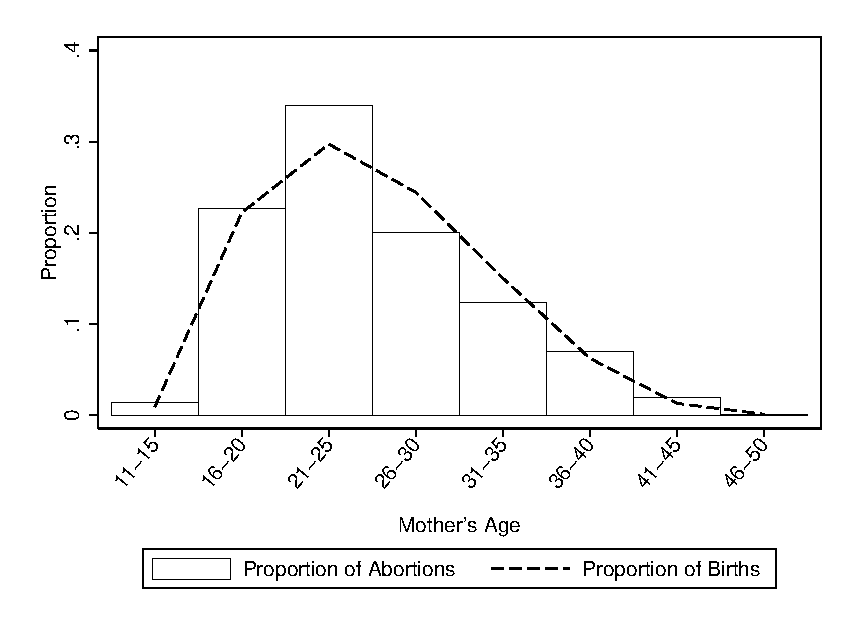
\includegraphics[scale=0.76]{graphs/birthDescriptives.eps}
  \caption{Birth and Abortion Descriptives: Mexico}
  \label{MexBirthAbort}
  \end{center}
  \vspace{2mm}
         {\footnotesize \textsc{Notes to figure}: Total births are plotted between
           2002 and 2011.
    Abortions are plotted from the date of reform (April 26, 2007) until 2011.
    The total quantity of births is 23.2 million (all of Mexico), and total
    abortions are 69,861 (Mexico City only).  Births are calculated from
    administrative data (INEGI) and abortions from administrative data (Secretary
    of Health, Mexico DF).}
\end{figure}
\vspace{2cm}


%\input{tables/MMR-wRegressive.tex}
%\input{tables/MMR-entropyWt.tex}
\input{tables/Births-unweight.tex}
\begin{landscape}
  \input{tables/Births-wild.tex}
\end{landscape}
\begin{landscape}
  \input{tables/Births-byAge.tex}
\end{landscape}


\begin{figure}[htpb!]
  \caption{Age-Specific Entropy-Weighted Trends in Births}
  \begin{center}
    \begin{subfigure}{0.45\textwidth}
      \includegraphics[scale=0.52]{graphs/entropyBirths_age15-18.eps}
      \caption{15-18 Year-olds}
    \end{subfigure}
    \begin{subfigure}{0.45\textwidth}
      \includegraphics[scale=0.52]{graphs/entropyBirths_age19-24.eps}
      \caption{19-24 Year-olds}
    \end{subfigure}
    \begin{subfigure}{0.45\textwidth}
      \includegraphics[scale=0.52]{graphs/entropyBirths_age25-34.eps}
      \caption{25-34 Year-olds}
    \end{subfigure}
    \begin{subfigure}{0.45\textwidth}
      \includegraphics[scale=0.52]{graphs/entropyBirths_age35-39.eps}
      \caption{35-39 Year-olds}
    \end{subfigure}
  \end{center}
  \textsc{Notes:} Refer to notes to figure \ref{fig:entropyBirth}.
  Entropy weights are calculated use pre-reform birth trends for
  the age group in each particular figure only.
\end{figure}



%\clearpage
%\input{tables/MXFLS_HHdecision_fetrend.tex}
%\input{tables/MXFLS_HHdecision_fetrend_placebo.tex}


\clearpage
\section{Correction for FWER Using Romano and Wolf's Stepdown Procedure}
\label{app:RomanoWolf}
We are interested in testing $K$ hypotheses regarding the effect of the
reforms on particular indicators.  As we are running multiple hypothesis
tests, the probability of falsely rejecting a null given that it is true
is high.  If we set the accepted type I error rate for each individual
hypothesis as $\alpha$, the likelihood of rejecting at least one
hypothesis incorrectly would be equal to $1-(1-\alpha)^K$ (assuming
independent hypotheses). For a type I error rate of $\alpha=0.05$ per
individual hypothesis and $K=5$ hypotheses, the likelihood of falsely
rejecting at least 1 null is thus equal to $\alpha_K=0.226$.

In order to proceed with testing we thus aim to fix the Family Wise Error
Rate (FWER), rather than the probability of type I errors for each
hypothesis individually.  This FWER is the probability of making at least
one type I error in the family of $K$ hypotheses, and we would like to fix
this value at $\alpha_K=0.05$.  The classical multiple hypothesis correction
of \citet{Bonferroni1935} suggests simply adjusting a constant correction
to inflate all p-values associated with each of the $K$ tests, however as
is well-known, this testing procedure is overly conservative, resulting
in low power \citep{RomanoWolf2005b}.  A more powerful series of tests
which both fix the FWER and have greater power are step-down methods, first
proposed by \citet{Holm1979}.  We follow a step-wise testing procedure
which is more powerful in terms of type II errors than classical multiple
hypothesis testing procedures given that it accounts for dependence between
hypothesis tests.  This stepdown procedure from \citet{RomanoWolf2005}, is
being increasingly used in empirical economics, see for example
\citet{SavelyevTan2015}.

We implement the ``Studentized StepM Method'' described in
\citet{RomanoWolf2005b} (p.\ 1252).  Specifically, we proceed
following the steps below, where the computationally intensive steps 1
and 2 need only be estimated once.
\begin{enumerate}
\item Estimate the $K$ models associated with each of the $K$ hypotheses and calculate the $t$-statistics associated with each hypothesis as $t_k=(\widehat\beta_k-\beta_k^{0})/se(\widehat\beta_k)$. Rank the absolute value of the $t_k$-statistics, and take the highest $t$-statistic to indicate the variable of interest for testing
\item Estimate $B=150$ bootstrap replications of each of the $K$ models, storing the t-statistic associated with each of the $K$ tests for each of the $B$ trials, resulting in $t_{k,b}$ t-statistics.  Also calculate the (bootstrap) standard error for each variable using the distribution of parameters across each of the $B$ bootstrap samples for a particular $k$.
\item For the variable of interest for testing, form the null distribution of $t$-statistics by taking the maximum $t$-statistic for each of the $B$ bootstrap replications among all of the potential donor variables.  The null distribution is defined as $t^{null}_{k}=|(\max(t)-\overline{\max(t)})/se(\widehat\beta_k)|$
\item Calculate the Romano Wolf $p$-value by comparing $t_k$ from step one with $t^{null}_k$ from step 3.  Store this $p$-value as the $p$-value corresponding to this variable.
\item Remove this variable from the list of variables to test, and remove the bootstrap replications associated with this variable from the pool of $t$-values for the null distribution.  The variable with the next highest $t$-statistic from 1 now becomes the variable of interest for testing, and the donor variables consist of this and the remaining variables to be tested.  If there remain variables to test, return to step 3.  Otherwise, end.
\end{enumerate}
\end{spacing}
\end{document}
